% Probability Formula Sheet
% ...place in a new file, e.g., probability_formula_sheet.tex

\documentclass[8pt]{article}
\usepackage{amsmath}
\usepackage{amssymb}
\usepackage[
    left=0.5in,
    right=0.5in,
    top=0.5in,
    bottom=0.5in
]{geometry}
\usepackage{graphicx}
\usepackage{color}
\usepackage{multicol} % Added for two columns
\usepackage{tabularx} % For better tables
\usepackage{array}    % For column formatting

\setlength{\parindent}{0pt}
% \setlength{\parskip}{0pt}
\def\chpiv@path{../../Chp 4}

\begin{document}

\begin{center}
    {\LARGE \textbf{MA213 Quiz 2 Formula Sheet}}
\end{center}

\vspace{1em}


\begin{multicols}{2} % Begin two columns

\textbf{Basic Probability Rules}
\begin{align*}
    &0 \leq P(A) \leq 1 \\
    &P(\text{Sample space}) = 1 \\
    &P(\text{not } A) = 1 - P(A) \qquad \text{(Complement rule)}
\end{align*}

\textbf{Addition Rules}
\begin{align*}
    &P(A \text{ or } B) = P(A) + P(B) \qquad \text{if $A$, $B$ disjoint} \\
    &P(A \text{ or } B) = P(A) + P(B) - P(A \text{ and } B) \qquad \text{Always}
\end{align*}

\textbf{Multiplication Rules}
\begin{align*}
    &P(A \text{ and } B) = P(A) \times P(B) \qquad \text{if $A$, $B$ independent} \\
    &P(A \text{ and } B) = P(A|B) \times P(B) \qquad \text{Always}
\end{align*}

\textbf{Conditional Probability}
\begin{align*}
    &P(A|B) = \frac{P(A \text{ and } B)}{P(B)} 
\end{align*}

\textbf{Law of Total Probability}
\[
P(B) = \sum_{i=1}^k P(B|A_i)P(A_i)
\]
where $A_1, \ldots, A_k$ partition the sample space.

\textbf{Bayes' Theorem}
\[
P(A|B) = \frac{P(B|A)P(A)}{P(B)}
\]
% or, if $A_1, \ldots, A_k$ partition the sample space,
% \[
% P(A_j|B) = \frac{P(B|A_j)P(A_j)}{\sum_{i=1}^k P(B|A_i)P(A_i)}
% \]

\textbf{Expected Value and Variance (Discrete)}
\begin{align*}
    &E(X) = \sum_{i} x_i P(X = x_i) \\
    &\mathrm{Var}(X) = \sum_{i} (x_i - E(X))^2 P(X = x_i)
\end{align*}

\textbf{Linear Combinations of Random Variables}

$X$, $Y$ random variables. $a$, $b$, $c$ constants.
\begin{align*}
    &E(aX + bY + c) = aE(X) + bE(Y) + c \qquad \text{Always} \\
    &\mathrm{Var}(aX + bY +c) = a^2\mathrm{Var}(X) + b^2\mathrm{Var}(Y) \quad \text{if } X, Y \text{ independent}
\end{align*}

% Add common distributions here
\textbf{Common Distributions}

\textit{Normal($\mu,\sigma^2$):}
\begin{align*}
    &E(X) = \mu \qquad \mathrm{Var}(X) = \sigma^2 \\
\end{align*}

\vspace{-2em}
if $X \sim \text{Normal}(\mu, \sigma^2)$, then $Z = \frac{X - \mu}{\sigma} \sim \text{Normal}(0,1)$

\begin{center}
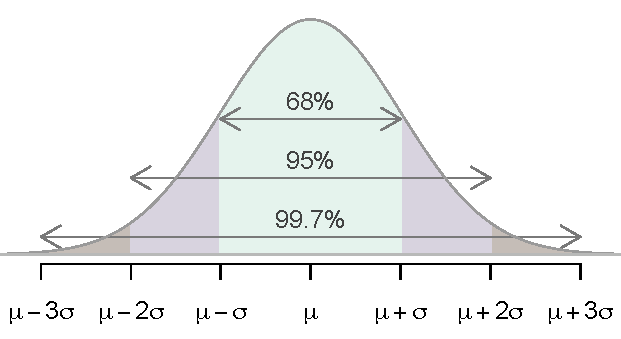
\includegraphics[width=0.3\textwidth]{\chpiv@path/4-1_normal_distribution/figures/6895997/6895997}
\end{center}

\textit{Bernoulli($p$):}
\begin{align*}
    &P(X = x) = p^x (1-p)^{1-x},\quad x=0,1 \\
    &E(X) = p \qquad \mathrm{Var}(X) = p(1-p)
\end{align*}

\textit{Geometric($p$):}
\begin{align*}
    &P(X = k) = (1-p)^{k-1}p,\quad k=1,2,\ldots \\
    &E(X) = \frac{1}{p} \qquad \mathrm{Var}(X) = \frac{1-p}{p^2}
\end{align*}

\textit{Binomial($n,p$):}
\begin{align*}
    &P(X = k) = \binom{n}{k}p^k(1-p)^{n-k},\quad k=0,\ldots,n \\
    &E(X) = np \qquad \mathrm{Var}(X) = np(1-p)\\
    &\text{if } np \ge 10 \text{ and } n(1-p) \ge 10, \\
    &\hspace{2em}\text{ then } X \sim \text{Binomial}(n,p) \approx \text{Normal}(np, np(1-p))
\end{align*}


\textit{Poisson($\lambda$):}
\begin{align*}
    &P(X = k) = \frac{\lambda^k e^{-\lambda}}{k!},\quad k=0,1,2,\ldots \\
    &E(X) = \lambda \qquad \mathrm{Var}(X) = \lambda
\end{align*}


\end{multicols} % End two columns

\vspace{1em}

% R Functions Table
\begin{center}
\renewcommand{\arraystretch}{1.3}
\begin{tabularx}{0.6\textwidth}{|>{\raggedright\arraybackslash}X|>{\raggedright\arraybackslash}X|}
\hline
\textbf{Distribution} & \textbf{R Functions} \\
\hline
Normal & \texttt{rnorm}, \texttt{dnorm}, \texttt{pnorm}, \texttt{qnorm} \\
\hline
Geometric & \texttt{rgeom}, \texttt{dgeom}, \texttt{pgeom}, \texttt{qgeom} \\
\hline
Binomial & \texttt{rbinom}, \texttt{dbinom}, \texttt{pbinom}, \texttt{qbinom} \\
\hline
Poisson & \texttt{rpois}, \texttt{dpois}, \texttt{ppois}, \texttt{qpois} \\
\hline
\end{tabularx}

\vspace{0.5em}
\textbf{r} -- generate random number; \textbf{d} -- PDF or PMF; \textbf{p} -- CDF; \textbf{q} -- inverse CDF
\end{center}

\end{document}